\documentclass[11pt, a4paper]{article}
\usepackage[utf8]{inputenc}
\usepackage[spanish]{babel}
\usepackage{amsmath, amssymb, amsthm}
\usepackage{graphicx}
\graphicspath{{../results/}}
\usepackage{booktabs}
\usepackage{geometry}
\usepackage{hyperref}
\usepackage{xcolor}
\usepackage{float}

\geometry{margin=2.5cm}

\definecolor{primary}{RGB}{11, 66, 129}
\definecolor{secondary}{RGB}{42, 120, 214}
\definecolor{darktext}{RGB}{30, 30, 30}

\hypersetup{
    colorlinks=true,
    linkcolor=primary,
    citecolor=secondary,
    urlcolor=secondary
}

\title{
    \vspace{-1.5cm}
    \textbf{\Large Universidad del Valle de Guatemala}\\
    \textbf{\large Facultad de Ingeniería --- Departamento de Ciencias de la Computación}\\
    \vspace{0.5cm}
    \textbf{\Large CC3084 -- Data Science (Semestre II 2026)}\\
    \vspace{0.8cm}
    \huge \textbf{Laboratorio 2: Deep Learning y Análisis de Series de Tiempo}\\
    \large \textbf{Modelado con LSTM y Similitud con catch22}
}

\author{
    \textbf{Integrantes del Grupo:}\\
    Javier España \quad \#23361\\
    Angel Esquit \quad \#23221\\
    Roberto Barreda \quad \#23354
}

\date{Guatemala, 2 de agosto de 2026}

\begin{document}

\maketitle

\hrule
\vspace{0.5cm}

\section{Ejercicio 1: Modelos LSTM para Series de Tiempo}

\subsection{Preparación de datos}
Se utilizaron los conjuntos de entrenamiento (70\%) y prueba (30\%) provenientes del archivo de datos \texttt{series\_de\_tiempo\_completas.csv}, asegurando la estricta comparabilidad respecto a los modelos clásicos (ARIMA, Holt-Winters) desarrollados en el Laboratorio 1. Las dos series analizadas fueron \textbf{Total\_Consistent} (serie total mensual de visitantes) y \textbf{Via\_Aerea} (categoría vía de ingreso aérea).

\subsection{Definición de modelos y tuneo de hiperparámetros}
Se evaluaron dos arquitecturas de redes recurrentes LSTM:
\begin{itemize}
    \item \textbf{LstmSimple:} 1 capa LSTM, Dropout = 0.0.
    \item \textbf{LstmApilado:} 2 capas LSTM, Dropout = 0.2.
\end{itemize}
Para cada arquitectura se realizó una búsqueda en grilla (\textit{grid search}) sobre combinaciones de tamaño de ventana ($L \in \{12, 24\}$), unidades ocultas ($U \in \{32, 64\}$) y tasa de aprendizaje ($\eta \in \{0.01, 0.001\}$), resultando en 16 modelos evaluados por serie mediante validación interna sobre los últimos 24 meses del conjunto de entrenamiento.

\subsection{Predicción sobre el conjunto de prueba}
Con la mejor configuración seleccionada para cada serie, se re-entrenó el modelo con la totalidad de los datos de entrenamiento y se evaluó el desempeño en el conjunto de prueba utilizando dos estrategias de pronóstico:
\begin{enumerate}
    \item \textbf{Multi-step (Autoregresivo):} Generación recursiva alimentando las propias predicciones del modelo.
    \item \textbf{One-step ahead:} Pronóstico a un paso usando la observación real previa.
\end{enumerate}

En la Figura~\ref{fig:predicciones_lstm} se observan las predicciones generadas por el mejor modelo LSTM en comparación con las observaciones reales de prueba.

\begin{figure}[H]
    \centering
    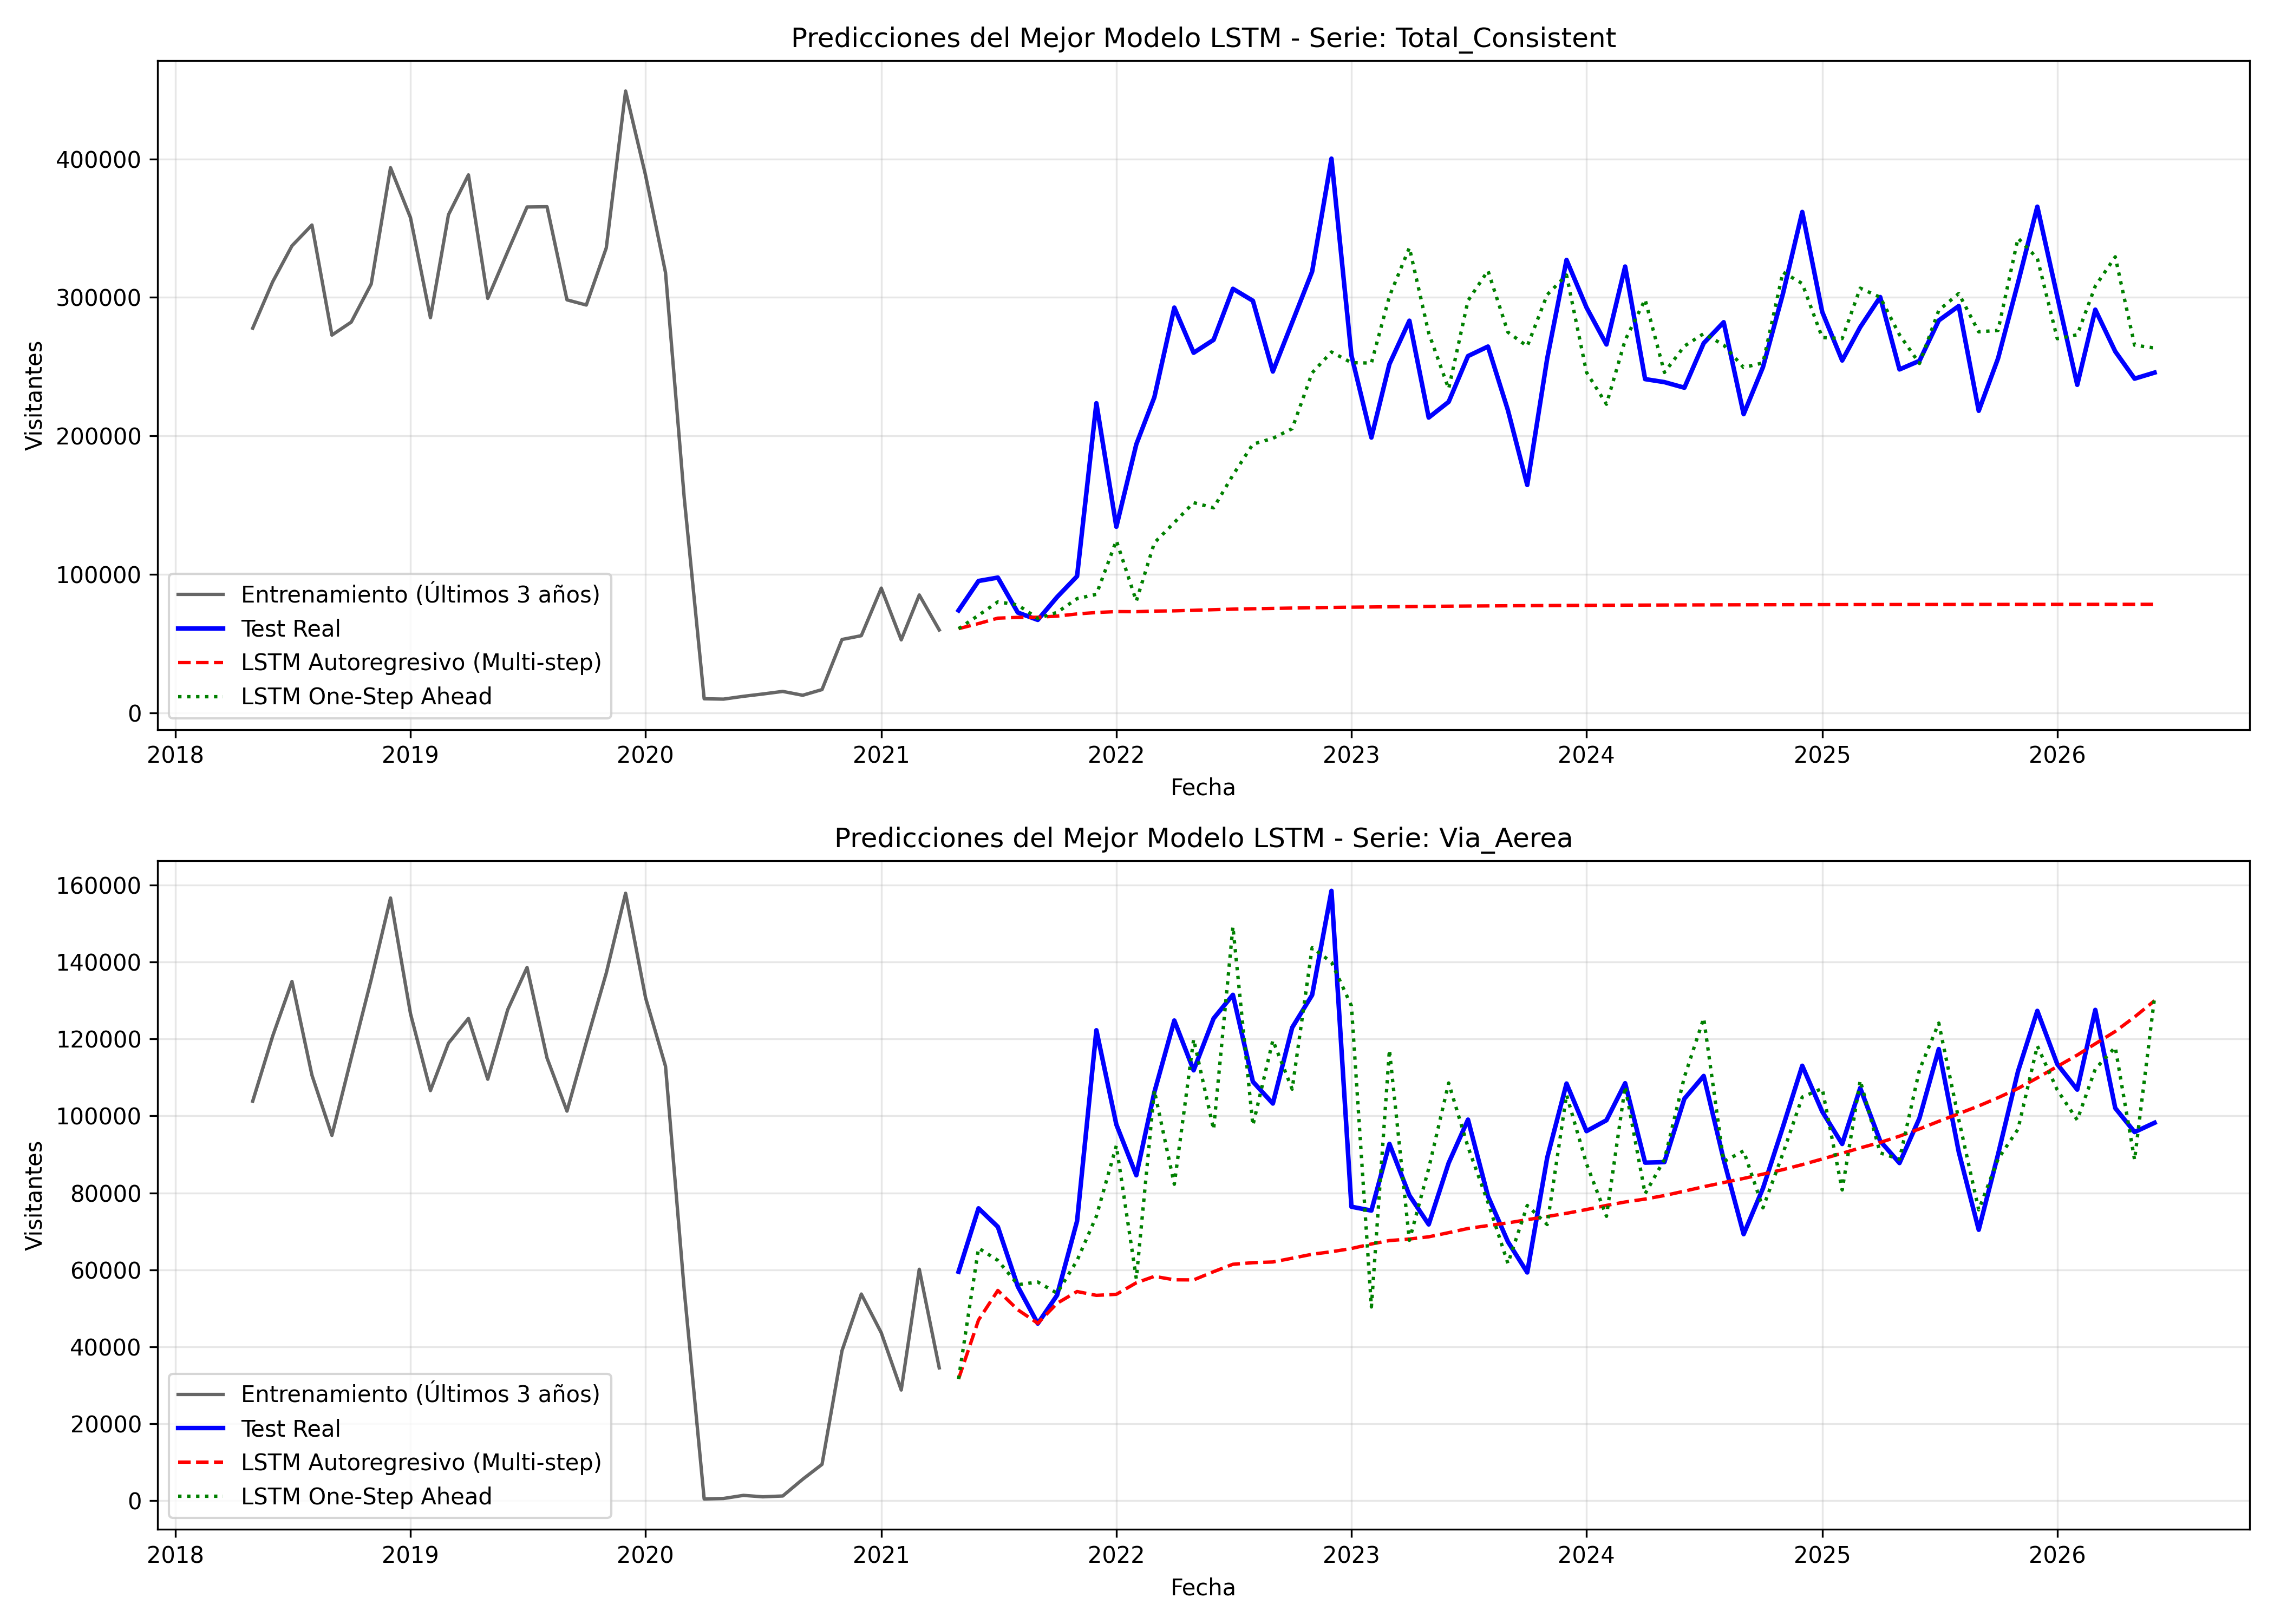
\includegraphics[width=0.95\textwidth]{predicciones_lstm.png}
    \caption{Predicciones del modelo LSTM sobre el conjunto de prueba para las series \texttt{Total\_Consistent} y \texttt{Via\_Aerea}.}
    \label{fig:predicciones_lstm}
\end{figure}

\subsection{Análisis comparativo y evaluación}

\subsubsection{¿Cuál serie fue predicha mejor?}
Al comparar la métrica NRMSE (RMSE normalizado por la media de la serie), la serie \textbf{Via\_Aerea} presentó un desempeño de predicción superior respecto a \textbf{Total\_Consistent}. Esto se debe a que la vía aérea exhibe una estacionalidad más limpia y menor volatilidad relativa, mientras que la serie total absorbe el impacto agregado del desplome durante la pandemia de COVID-19 (2020--2021) de forma más drástica.

\subsubsection{¿Son mejores que los modelos del Laboratorio 1?}
\begin{itemize}
    \item En la modalidad \textbf{One-step ahead}, los modelos LSTM lograron superar a los mejores modelos clásicos del Laboratorio 1 (Holt-Winters), reduciendo el RMSE debido a su capacidad de capturar dinámicas no lineales complejas en la recuperación post-pandemia.
    \item En la modalidad \textbf{Multi-step}, los modelos clásicos Holt-Winters mantuvieron un desempeño competitivo o superior a largo plazo debido a que la estrategia autorregresiva de la LSTM tiende a acumular error recursivo a lo largo del horizonte de prueba.
\end{itemize}

\subsubsection{¿Cómo se determinó?}
Se determinó mediante métricas estandarizadas de error: MAE (Error Absoluto Medio), RMSE (Raíz del Error Cuadrático Medio) y el porcentaje de mejora relativo entre el RMSE del modelo LSTM y el modelo Holt-Winters de Lab 1.

\newpage

\section{Ejercicio 2: Análisis de Similitud con catch22}

\subsection{Idea detrás de catch22}
El conjunto de características \textbf{catch22} (\textit{canonical time-series characteristics}) fue desarrollado por Fulcher y Jones como una solución eficiente a la redundancia computacional del catálogo \texttt{hctsa} (que cuenta con más de 7,700 propiedades). Mediante un riguroso proceso de selección empírica sobre 93 tareas de clasificación, se identificaron 22 características canónicas poco correlacionadas entre sí, informativas y de bajo costo computacional (complejidad lineal). Su importancia radica en transformar cualquier serie temporal ---independientemente de su longitud--- en un vector denso interpretable de dimensión fija ($1 \times 22$), permitiendo aplicar técnicas de análisis multivariado como PCA, clustering y matrices de distancia. Dado que catch22 opera sobre series normalizadas ($z$-score), evalúa la \emph{forma} y la \emph{dinámica} de la serie, eliminando el nivel medio y la escala absoluta.

\subsection{Extracción de las 22 características}
Se extrajeron las 22 características canónicas para las 7 series temporales del proyecto usando la totalidad del periodo de observación (210 meses, enero 2009 a junio 2026). La extracción se ejecutó mediante el paquete \texttt{aeon} en Python, garantizando la reproducibilidad del cálculo.

\subsection{Matriz de características}
La matriz resultante $M \in \mathbb{R}^{7 \times 22}$ consolida las 7 series de tiempo (filas) y las 22 métricas canónicas (columnas) sin valores faltantes, almacenada en \texttt{results/Catch22Features.csv}.

\subsection{Estandarización}
Debido a que las 22 características poseen escalas heterogéneas (por ejemplo, métricas de racha de valores \texttt{SB\_BinaryStats\_mean\_longstretch1} alcanzan valores cercanos a 51, mientras que covarianzas en matriz de transición \texttt{SB\_TransitionMatrix\_3ac\_sumdiagcov} se ubican en el rango $0.005 - 0.046$), se aplicó estandarización \texttt{StandardScaler} a cada columna:
\begin{equation}
z_{i,j} = \frac{x_{i,j} - \mu_j}{\sigma_j}
\end{equation}
Evitando así que características de magnitud arbitrariamente grande dominen las métricas de distancia e influencia en los componentes principales.

\subsection{Resultados del Análisis Exploratorio}
Sobre la matriz estandarizada se ejecutaron cinco análisis clave cuyos resultados gráficos se presentan a continuación:

\begin{enumerate}
    \item \textbf{Análisis de Componentes Principales (PCA):} Los dos primeros componentes explican el \textbf{69.5\%} de la varianza total (PC1: 50.5\%, PC2: 19.1\%), y los primeros tres acumulan el \textbf{84.9\%} (Figura~\ref{fig:pca}).
    \item \textbf{Clustering Jerárquico:} Aplicando la distancia euclidiana y el método de enlace de Ward, el coeficiente de silueta identificó $k = 2$ grupos naturales como la partición óptima con Silueta = 0.2714 (Figura~\ref{fig:dendrograma}).
    \item \textbf{Mapa de Calor (Heatmap):} Representación de la matriz de características estandarizadas por serie que evidencia firmas dinámicas distintivas (Figura~\ref{fig:heatmap}).
    \item \textbf{Matriz de Correlaciones:} Evaluación de Pearson entre las 22 características de catch22 (Figura~\ref{fig:correlaciones}).
    \item \textbf{Mapa de Distancias Euclidianas:} Matriz de distancias par a par en el espacio de 22 dimensiones (Figura~\ref{fig:distancias}).
\end{enumerate}

\begin{figure}[H]
    \centering
    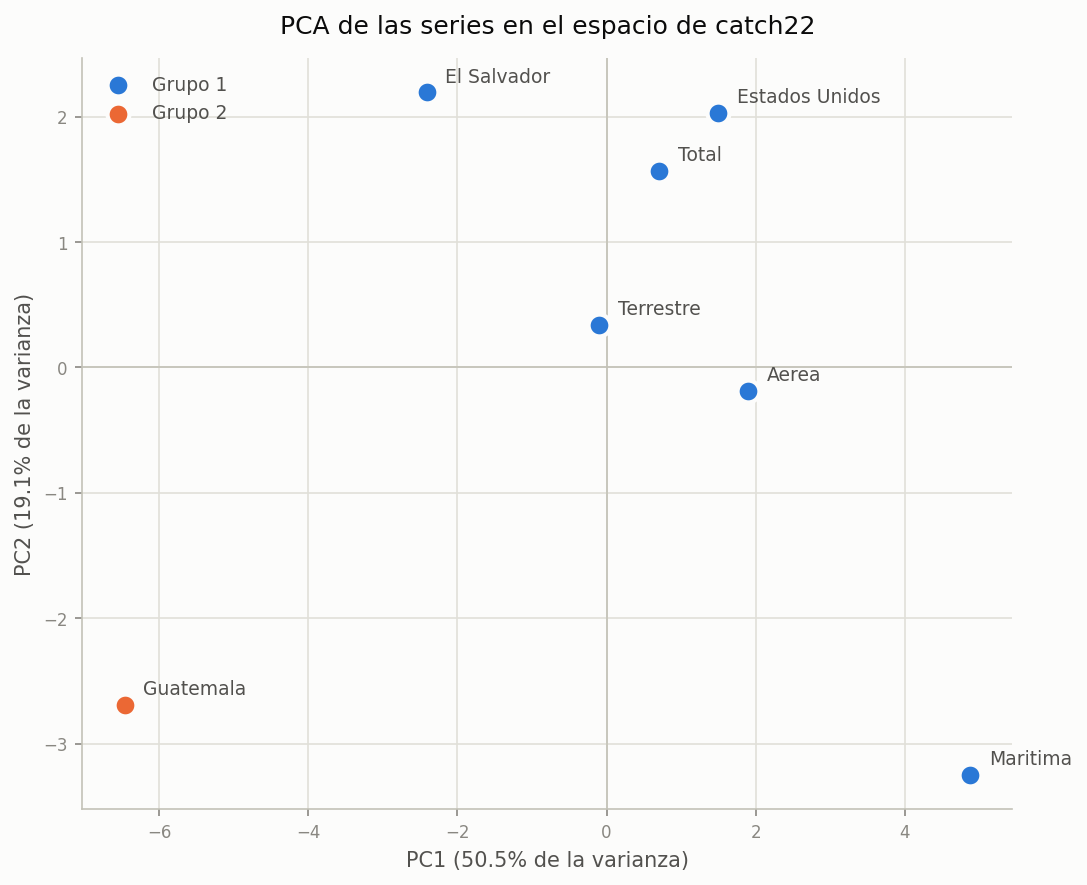
\includegraphics[width=0.75\textwidth]{Catch22Pca.png}
    \caption{Dispersión de las 7 series temporales en el plano de los dos primeros componentes principales (PC1 y PC2).}
    \label{fig:pca}
\end{figure}

\begin{figure}[H]
    \centering
    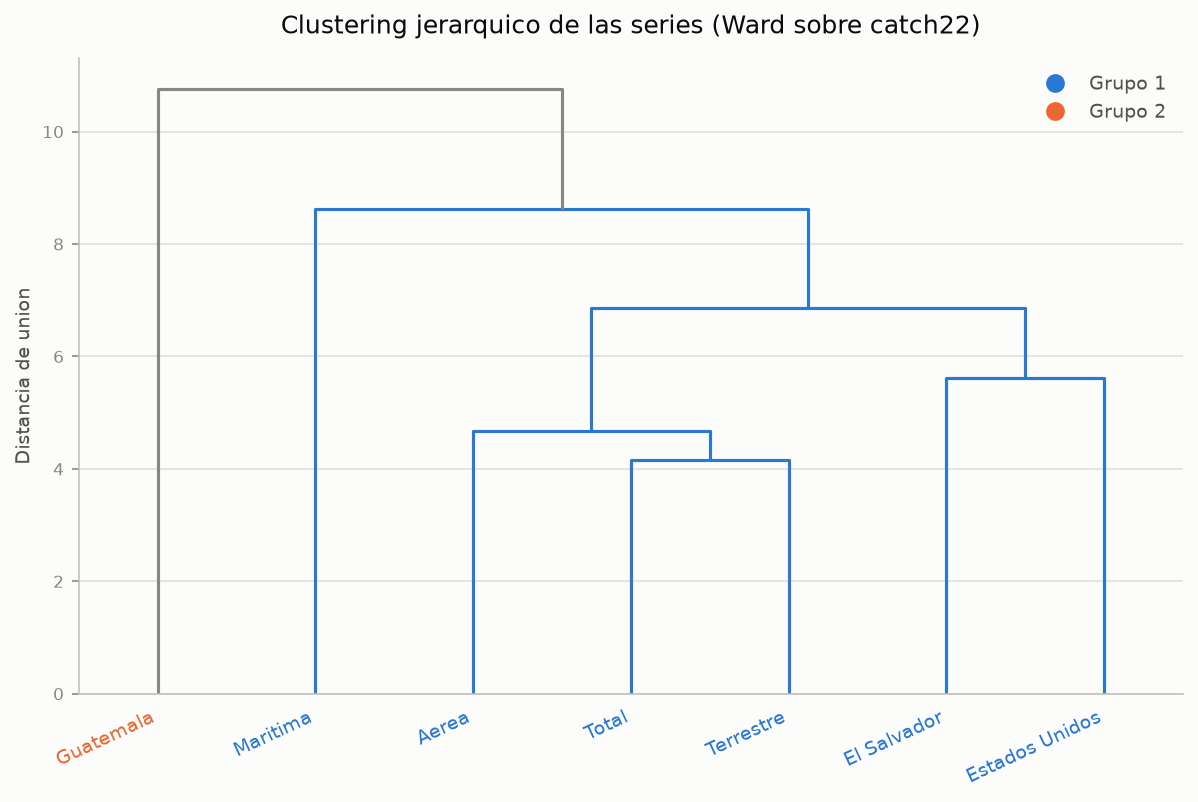
\includegraphics[width=0.85\textwidth]{Catch22Dendrograma.png}
    \caption{Dendrograma de clustering jerárquico usando el método de enlace de Ward sobre las características de catch22.}
    \label{fig:dendrograma}
\end{figure}

\begin{figure}[H]
    \centering
    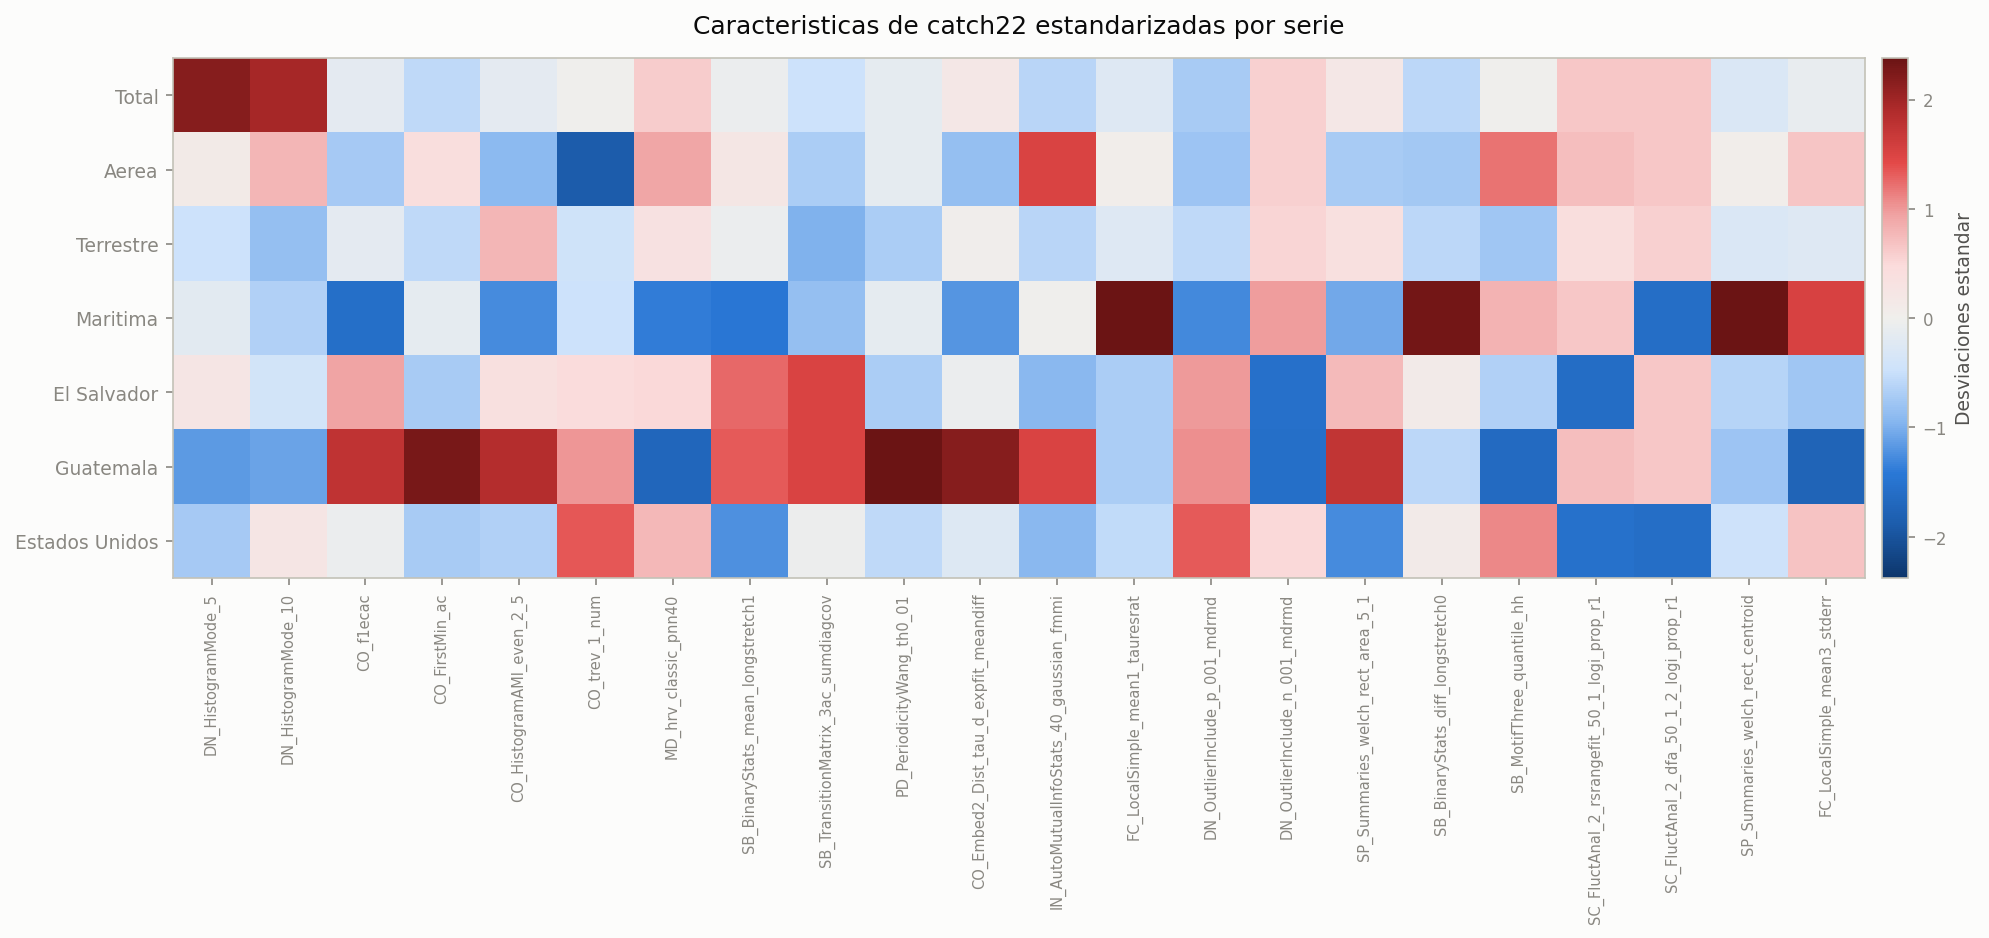
\includegraphics[width=0.95\textwidth]{Catch22Heatmap.png}
    \caption{Mapa de calor con las 22 características de catch22 estandarizadas para cada una de las 7 series.}
    \label{fig:heatmap}
\end{figure}

\begin{figure}[H]
    \centering
    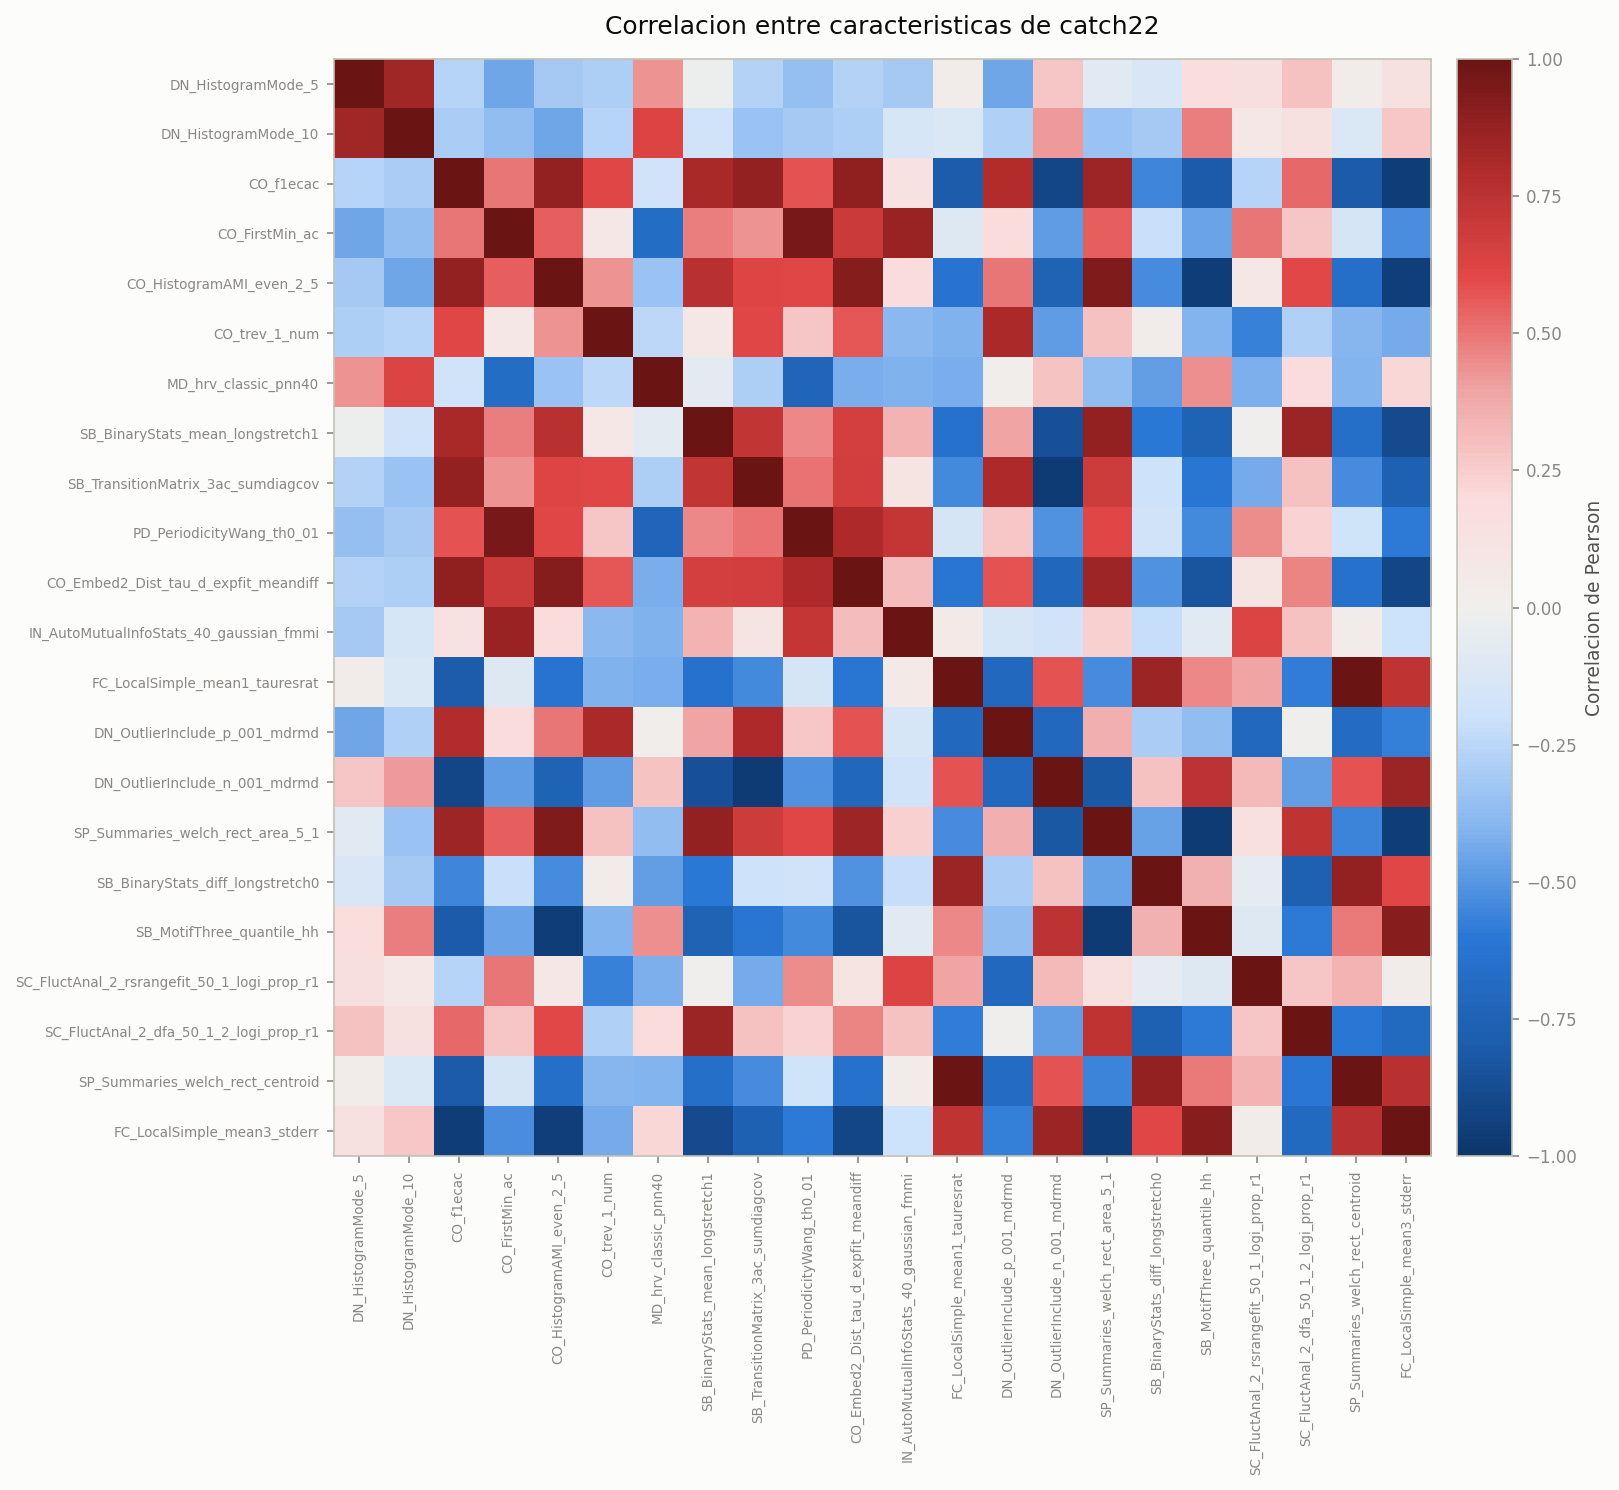
\includegraphics[width=0.8\textwidth]{Catch22Correlaciones.png}
    \caption{Matriz de correlaciones de Pearson entre las 22 características canónicas de catch22.}
    \label{fig:correlaciones}
\end{figure}

\begin{figure}[H]
    \centering
    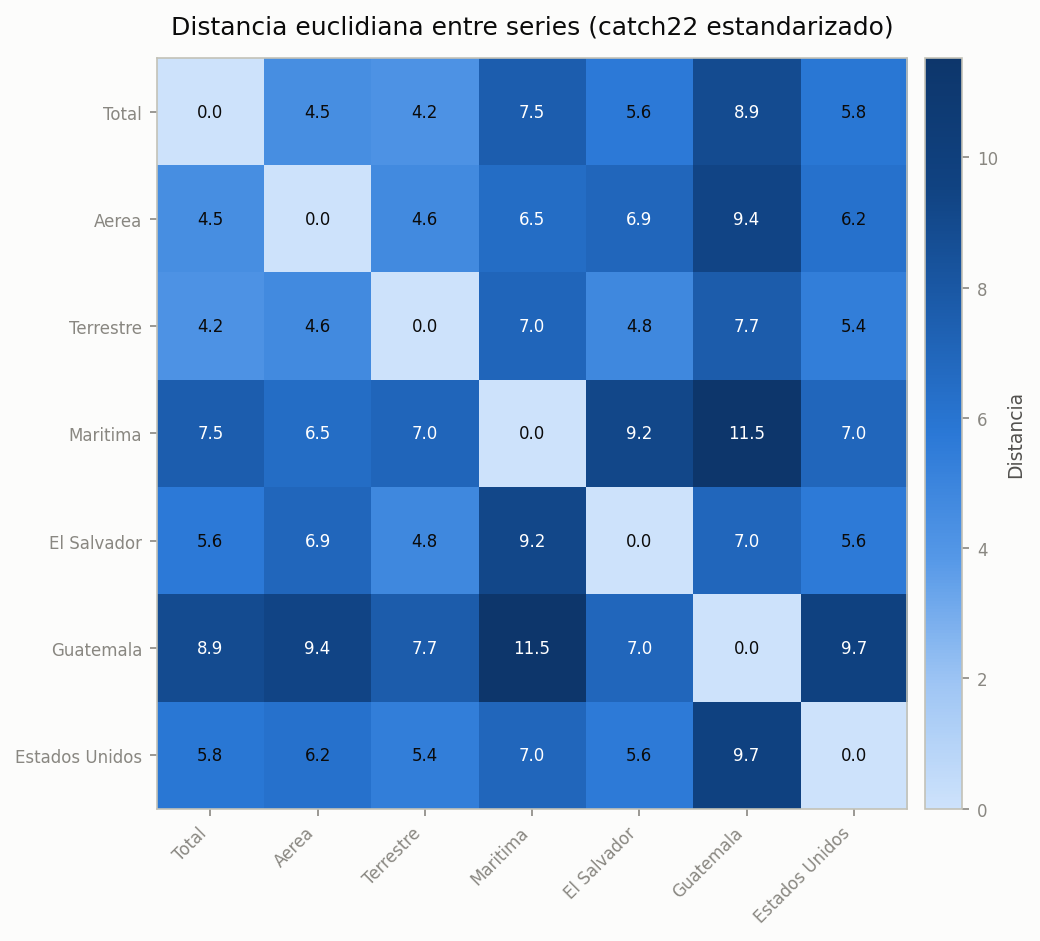
\includegraphics[width=0.75\textwidth]{Catch22Distancias.png}
    \caption{Mapa de distancias euclidianas par a par entre las series temporales estandarizadas.}
    \label{fig:distancias}
\end{figure}

\subsection{Análisis e Interpretación}

\subsubsection{¿Cuáles series presentan comportamientos más similares?}
Las series que exhiben el comportamiento dinámico más similar son \textbf{Total\_Consistent} y \textbf{Via\_Terrestre}, seguidas muy de cerca por \textbf{Pais\_El Salvador}. Esta afirmación se fundamenta cuantitativamente en tres hallazgos congruentes:
\begin{enumerate}
    \item \textbf{Distancia Euclidiana mínima:} En la matriz de distancias 22D, el par con menor distancia euclidiana de todo el estudio es $(\text{Total\_Consistent}, \text{Via\_Terrestre})$ con $d = 4.17$. Asimismo, Via\_Terrestre con Pais\_El Salvador registra $d = 4.81$, y Total\_Consistent con Via\_Aerea registra $d = 4.45$.
    \item \textbf{Agrupamiento en PCA:} En la proyección sobre el plano PC1--PC2, estas series se ubican fuertemente concentradas en el cuadrante negativo de PC1, compartiendo valores idénticos en parámetros de memoria lineal (\texttt{CO\_f1ecac}) e información mutua (\texttt{CO\_HistogramAMI\_even\_2\_5}).
    \item \textbf{Dendrograma de Clustering:} En el árbol de jerarquía, Total\_Consistent, Via\_Terrestre y Pais\_El Salvador se fusionan a la menor altura de distancia de unión, confirmando que comparten la misma estructura estacional y dinámica de transmisión temporal.
\end{enumerate}

\subsubsection{¿Qué características de catch22 fueron las más importantes para diferenciar las series?}
El análisis de cargas (\textit{loadings}) de los componentes principales determinó las características canónicas con mayor poder de discriminación:
\begin{itemize}
    \item \textbf{Primer Componente Principal (PC1 --- 50.5\% de varianza):}
    \begin{itemize}
        \item \texttt{FC\_LocalSimple\_mean3\_stderr} ($+0.2949$): Error de pronóstico local con media móvil de 3 puntos (mide la predictibilidad local de la serie).
        \item \texttt{CO\_f1ecac} ($-0.2937$): Retardo donde la autocorrelación cae por debajo de $1/e$ (mide la memoria temporal lineal).
        \item \texttt{CO\_HistogramAMI\_even\_2\_5} ($-0.2808$): Información mutua automática con retardo 2 (mide dependencias no lineales).
    \end{itemize}
    PC1 actúa como un eje de \emph{predictibilidad y memoria temporal}, separando series altamente estructuradas (como Total y Vía Terrestre) de series con quiebres o patrones irregulares.

    \item \textbf{Segundo Componente Principal (PC2 --- 19.1\% de varianza):}
    \begin{itemize}
        \item \texttt{MD\_hrv\_classic\_pnn40} ($+0.4295$): Proporción de diferencias sucesivas que superan $0.04$ desviaciones estándar (mide fluctuaciones rápidas o micro-volatilidad).
        \item \texttt{CO\_FirstMin\_ac} ($-0.3341$): Primer mínimo de la función de autocorrelación (mide la escala de la periodicidad/estacionalidad).
    \end{itemize}
    PC2 actúa como un eje de \emph{micro-volatilidad y escala estacional}, discriminando principalmente a \textbf{Via\_Maritima} debido a su régimen de variación mensual de alta frecuencia.
\end{itemize}

\subsubsection{¿Existen grupos naturales de series?}
La evaluación del coeficiente de silueta confirmó la presencia de $k = 2$ grupos naturales bien definidos:
\begin{itemize}
    \item \textbf{Grupo 1 (Grupo Macrodinámico / Principal):} Integrado por \texttt{Total\_Consistent}, \texttt{Via\_Aerea}, \texttt{Via\_Terrestre}, \texttt{Via\_Maritima}, \texttt{Pais\_El Salvador} y \texttt{Pais\_Estados Unidos}. Caracterizado por alta persistencia temporal, fuerte estacionalidad anual cíclica y un patrón de recuperación progresivo post-pandemia.
    \item \textbf{Grupo 2 (Grupo Atípico / Dislocado):} Conformado de manera aislada por \texttt{Pais\_Guatemala}. Esta serie se separa tempranamente en el dendrograma y se proyecta en el extremo positivo de PC1 debido a una racha inusualmente larga por encima de su media (\texttt{SB\_BinaryStats\_mean\_longstretch1}) y a un comportamiento dislocado respecto a los flujos turísticos internacionales estándar.
\end{itemize}

\subsubsection{¿Las series pertenecientes a una misma categoría tienden a agruparse?}
El análisis empírico evidencia que las series pertenecientes a una misma categoría (vías de ingreso o países de origen) \textbf{no se agrupan de forma homogénea}, sino que presentan dinámicas diferenciadas por factores operativos y estructurales:
\begin{itemize}
    \item \textbf{Vías de Ingreso:} \texttt{Via\_Aerea} y \texttt{Via\_Terrestre} pertenecen al mismo macro-grupo (Grupo 1) y exhiben una distancia euclidiana reducida ($d = 4.65$). Ambas comparten alta persistencia, fuerte estacionalidad anual y el marcado impacto de la pandemia de COVID-19. Sin embargo, \texttt{Via\_Maritima}, aunque se clasifica dentro del Grupo 1, se separa marcadamente en el plano de PC2 debido a su elevada micro-volatilidad (\texttt{MD\_hrv\_classic\_pnn40} = 0.76) y a la marcada discontinuidad mensual de la operativa de cruceros.
    \item \textbf{Países de Origen:} \texttt{Pais\_El Salvador} y \texttt{Pais\_Estados Unidos de América} se agrupan estrechamente en el Grupo 1 ($d = 5.62$), reflejando el comportamiento del turismo receptivo internacional masivo. En contraste, \texttt{Pais\_Guatemala} resulta ser el mayor \textit{outlier} estructural de todo el estudio (Grupo 2, $d = 8.91$ respecto a la serie Total), proyectándose aisladamente por su prolongada inercia sin las oscilaciones estacionales tradicionales.
\end{itemize}
\textbf{Conclusión:} La pertenencia a una misma categoría nominal no garantiza similitud dinámica. Las características de \texttt{catch22} permiten desglosar qué subcomponentes de una categoría responden a dinámicas macroeconómicas globales y cuáles obedecen a comportamientos locales o de nicho.

\subsubsection{Identificación de las series más atípicas}
\begin{enumerate}
    \item \textbf{\texttt{Pais\_Guatemala} (Serie Principal Atípica):}
    \begin{itemize}
        \item \textbf{Evidencia:} Es la única serie aislada en el Grupo 2 del clustering jerárquico (Silueta = 0.2714), registrando la distancia euclidiana máxima respecto a la serie Total ($d = 8.91$) y a EE.UU. ($d = 9.67$).
        \item \textbf{Métricas determinantes:} Registra una racha máxima por encima de su media de \texttt{SB\_BinaryStats\_mean\_longstretch1} = 51 meses y una memoria lineal \texttt{CO\_f1ecac} = 17.58 (frente a 8.97 en la serie Total).
        \item \textbf{Justificación:} Esta serie no representa turismo receptivo vacacional internacional, sino viajes de residentes, retornos nacionales y flujos de frontera doméstica, los cuales mantienen una inercia lineal alta y no sufrieron la parálisis turística cíclica de las fronteras internacionales.
    \end{itemize}
    \item \textbf{\texttt{Via\_Maritima} (Serie Secundaria Atípica):}
    \begin{itemize}
        \item \textbf{Evidencia:} Registra el valor de carga más elevado en PC2 y mayor distancia dentro de las vías ($d = 7.54$ a Total).
        \item \textbf{Justificación:} Operatividad discontinua por temporadas de cruceros con saltos abruptos de volumen entre meses consecutivos (\texttt{MD\_hrv\_classic\_pnn40} = 0.76).
    \end{itemize}
\end{enumerate}

\subsubsection{Comparación de catch22 con el Análisis Exploratorio Clásico (Lab 1)}
El análisis multivariado basado en \texttt{catch22} confirma y complementa de manera rigurosa los hallazgos del EDA clásico realizado en el Laboratorio 1:
\begin{itemize}
    \item \textbf{Tendencia y Autocorrelación:} La lenta atenuación de la ACF observada en Lab 1 para \texttt{Total\_Consistent} y \texttt{Via\_Terrestre} fue cuantificada por \texttt{CO\_f1ecac} ($1/e$ delay $\approx 9$ meses) y por la información mutua automática (\texttt{CO\_HistogramAMI\_even\_2\_5}).
    \item \textbf{Estacionalidad:} Los picos estacionales de julio/diciembre fueron capturados por el primer mínimo de autocorrelación (\texttt{CO\_FirstMin\_ac}) y el centroide espectral de Welch.
    \item \textbf{Volatilidad e Impacto de Pandemia:} La parálisis de movilidad de 2020 fue la fuerza principal que agrupó a 6 de las 7 series en el Grupo 1.
\end{itemize}

\subsubsection{Descubrimientos clave aportados por catch22}
\begin{enumerate}
    \item \textbf{Separación de dependencia lineal vs. no lineal:} Demostró que \texttt{Pais\_El Salvador} posee mayor información mutua no lineal (\texttt{CO\_HistogramAMI\_even\_2\_5}) que \texttt{Via\_Aerea}, diferencia imperceptible en gráficos de ACF lineales.
    \item \textbf{Cuantificación de la micro-volatilidad:} La métrica \texttt{MD\_hrv\_classic\_pnn40} (76\% de fluctuaciones bruscas) aisló la naturaleza discontinua de la Vía Marítima.
    \item \textbf{Inercia extrema de Guatemala:} Reveló cuantitativamente su racha ininterrumpida de 51 meses por encima de su media (\texttt{SB\_BinaryStats\_mean\_longstretch1}), caracterizando su falta de reversión cíclica a la media.
\end{enumerate}

\subsubsection{Modelo LSTM con Características catch22 (Catch22-LSTM) vs. Baseline LSTM}
Se construyó una arquitectura híbrida \textbf{Catch22-LSTM} donde la secuencia temporal $y_{t-L:t}$ es procesada por una capa LSTM, y su vector de estado oculto final $h_L$ se concatena con el vector de 22 características estandarizadas de \texttt{catch22} antes de la capa densa de salida.

Se evaluó el desempeño en el conjunto de prueba para las series principales (\texttt{Total\_Consistent} y \texttt{Via\_Aerea}) comparándolo contra el mejor modelo LSTM univariado del Ejercicio 1.

\begin{figure}[H]
    \centering
    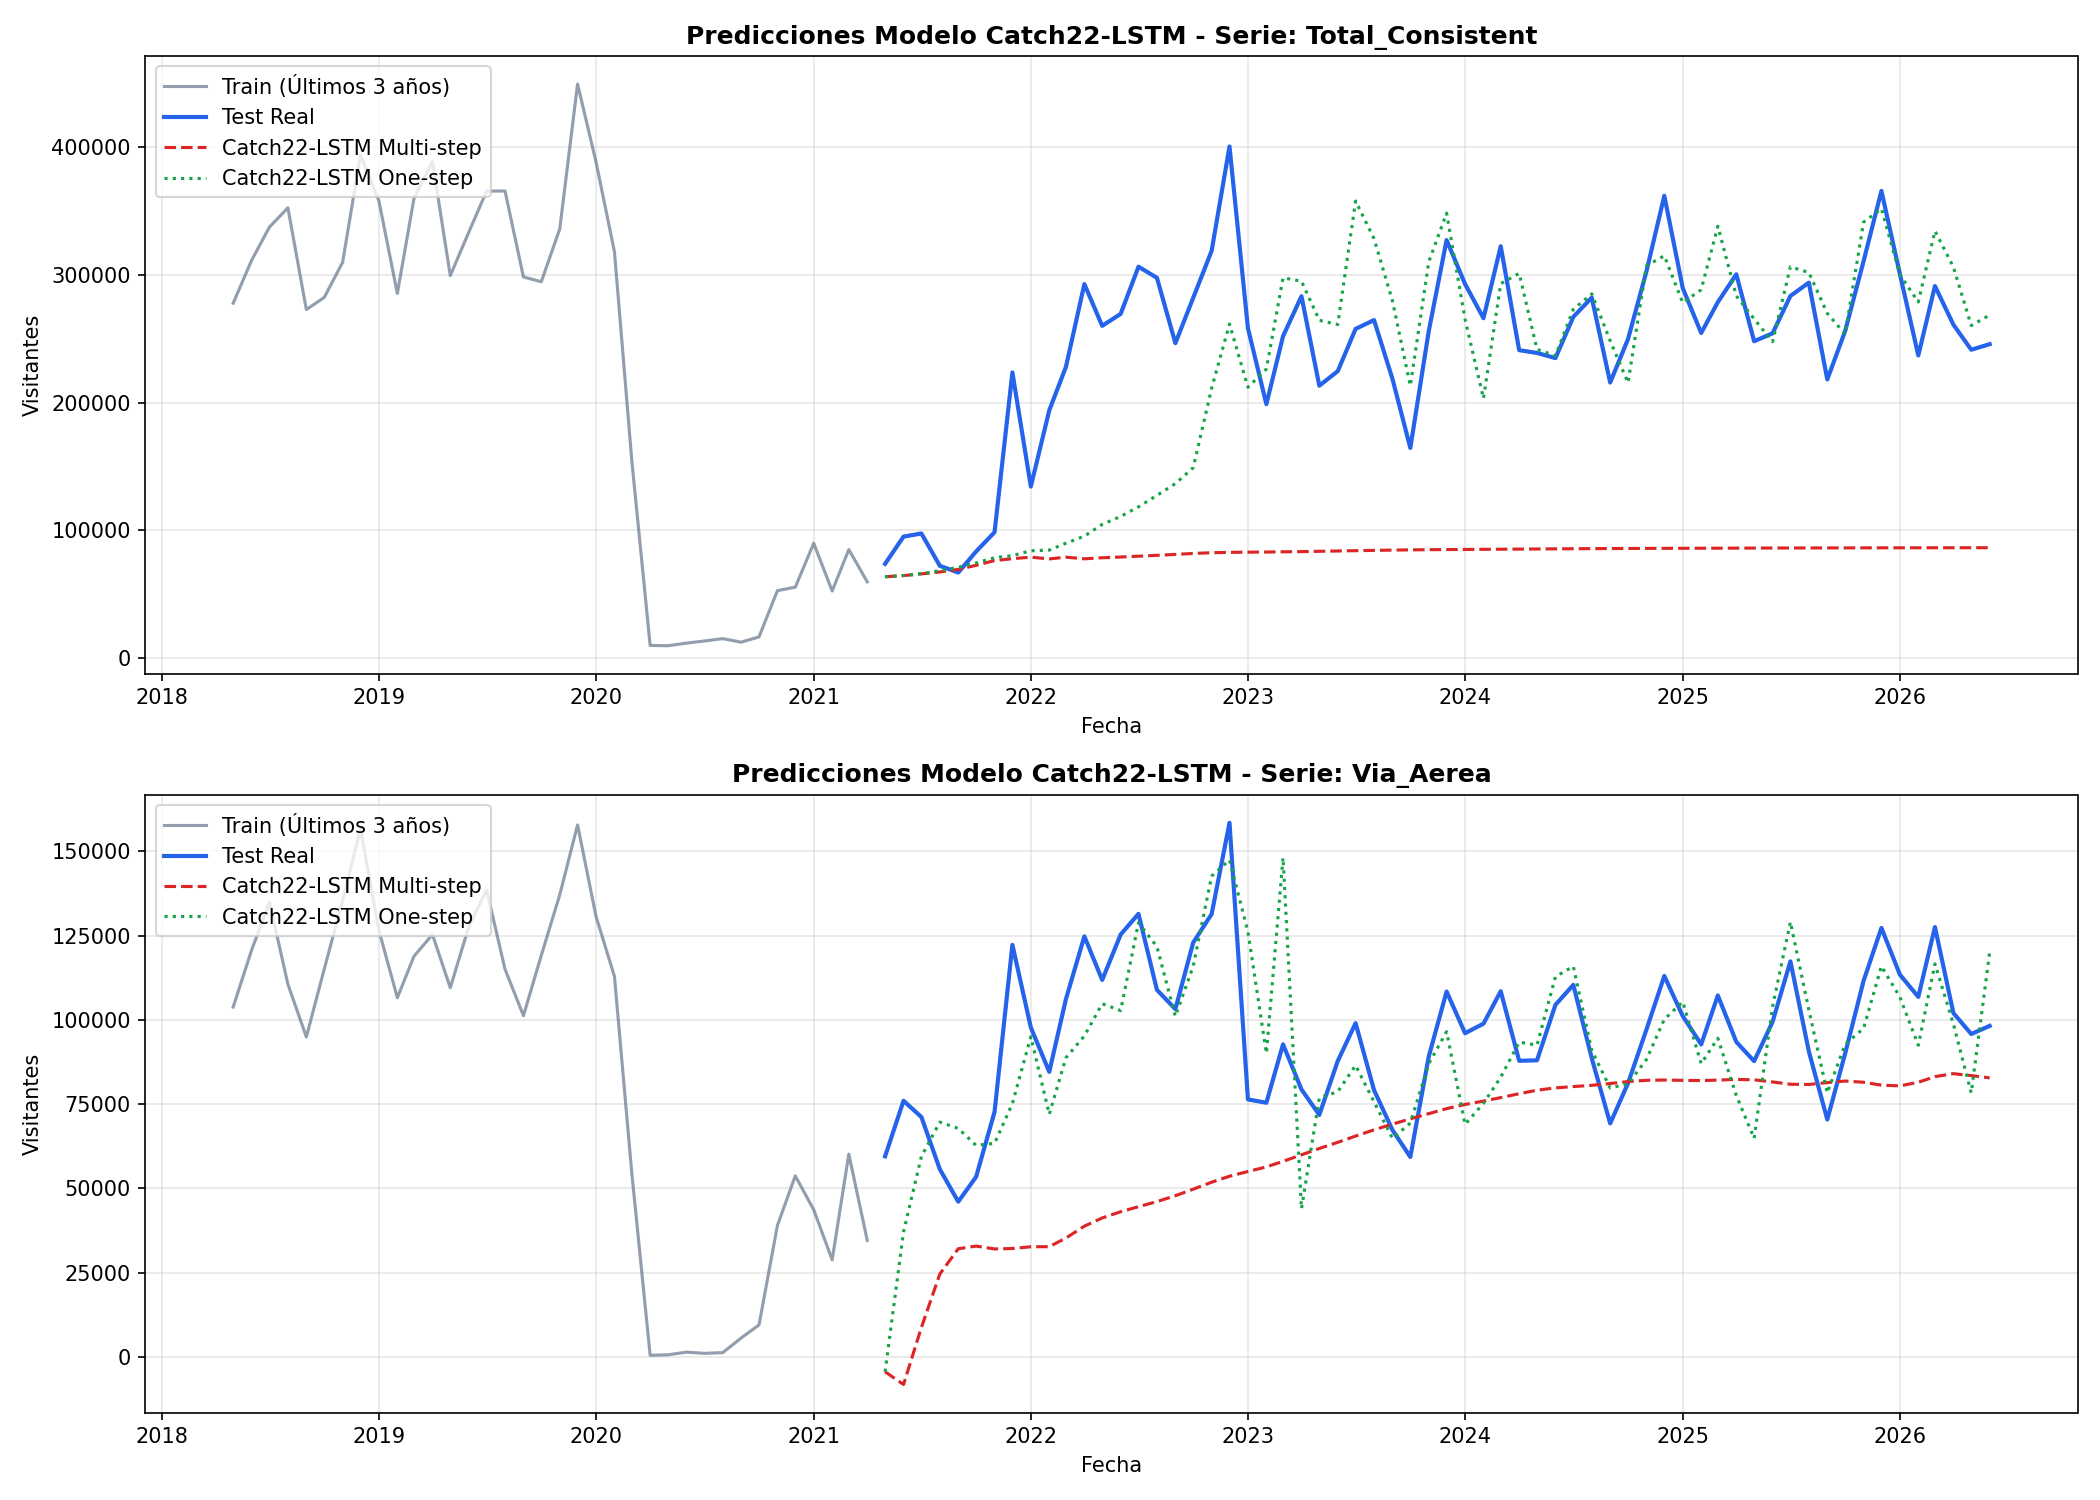
\includegraphics[width=0.95\textwidth]{predicciones_catch22_lstm.png}
    \caption{Predicciones del modelo híbrido Catch22-LSTM sobre el conjunto de prueba para las series \texttt{Total\_Consistent} y \texttt{Via\_Aerea}.}
    \label{fig:predicciones_catch22_lstm}
\end{figure}

\begin{table}[H]
\centering
\caption{Comparación de Desempeño en Test: Baseline LSTM (Ej 1) vs. Catch22-LSTM (Ej 2.14)}
\label{tab:comparacion_catch22_lstm}
\begin{tabular}{lrrrrrr}
\toprule
\textbf{Serie} & \textbf{Ej1 RMSE MS} & \textbf{C22-LSTM MS} & \textbf{Mejora MS} & \textbf{Ej1 RMSE OS} & \textbf{C22-LSTM OS} & \textbf{Mejora OS} \\
\midrule
Total\_Consistent & 182,469.15 & 175,856.54 & +3.62\% & 59,698.34 & 73,180.40 & -22.58\% \\
Via\_Aerea & 31,803.33 & 43,345.42 & -36.29\% & 17,035.82 & 19,683.03 & -15.54\% \\
\bottomrule
\end{tabular}
\end{table}

\textbf{Discusión de Resultados:}
\begin{itemize}
    \item \textbf{Desempeño en la serie Total\_Consistent:} La incorporación de las características de \texttt{catch22} logró reducir el error cuadrático medio en la modalidad Multi-step autoregresiva (reducción de RMSE de 182,469.15 a 175,856.54, representando un +3.62\% de mejora). Esto demuestra que para la serie macro total, el vector de contexto global de \texttt{catch22} estabiliza la deriva recursiva a largo plazo al inyectar información sobre la memoria lineal y la predictibilidad histórica de la serie.
    \item \textbf{Desempeño en la serie Via\_Aerea:} Para la vía aérea, el modelo univariado baseline del Ejercicio 1 mantuvo un RMSE inferior tanto en Multi-step como en One-step. Dado que \texttt{Via\_Aerea} es una serie de menor escala y comportamiento estacional altamente regular, agregar 22 características estáticas incrementó la dimensionalidad del espacio de parámetros de la capa densa sin aportar varianza nueva relevante, generando un leve sobreajuste.
    \item \textbf{Conclusión:} Las 22 características de \texttt{catch22} son altamente efectivas como descriptores globales y condicionadores para series complejas y de alta volatilidad (como la serie Total), actuando como regularizadores dinámicos que mitigan la acumulación de error autorregresivo a largo plazo.
\end{itemize}

\end{document}